\documentclass[12pt]{article}
\usepackage[french]{babel}
\usepackage[utf8]{inputenc}
\usepackage{amsmath}
\usepackage{amssymb}
\usepackage{tikz}
\usepackage{tkz-tab}
\usepackage{xcolor}
\usepackage{graphicx}
\usepackage{geometry}
\geometry{a4paper, margin=1in}

\title{DS commun Sujet A}
\author{Lycée Jacques Decour - Seconde 2025-2026}
\date{}

\begin{document}

\maketitle

{\color{red}
\underline{\textbf{(À LIRE) Remarques générales :}}

\vspace{5pt}
\begin{itemize}
    \item Ce devoir est important, il rassemble beaucoup de notions à maîtriser pour l'an prochain (spé 
    ou pas). Je compte sur vous pour retravailler les exos ratés cet été (au moins quelques heures)

    \vspace{5pt}
    \item Le \textbf{barème} apparaît ici sur chaque question 
    
    \vspace{5pt}
    \item beaucoup d'erreurs de calculs ! À retravailler : développement, factorisation, identités 
    remarquables etc...

    \vspace{5pt}
    \item Attention : on additionne pas des $x$ avec des nombres ! Ni les $x^2$, ce sont des 
    familles différentes : par exemple $2x + 3 + x^2 - 2 = 2x + x^2 + 1$ et on laisse comme ça !
    
    \vspace{5pt}
    \item Exo 1 c) : il n'y a pas de parenthèses autour de $\dfrac{3}{2}x - 4$ donc on ne 
    \textbf{distribue pas} le $\dfrac{3}{2}x$ dans la parenthèse !! Uniquement le $-4$.

    \vspace{5pt}
    \item Beaucoup d'erreurs sur les inéquations simples (question 2)a) de l'exo 3), on résout simplement en isolant 
    $x$ !

    \vspace{5pt}
    \item Très peu de gens ont résolu correctement l'inéquation quotient. Il y a une méthode dans le cours pour ce genre 
    d'inéquation ! Il faut \textbf{obligatoirement un tableau de signes}

    \vspace{5pt}
    \item Encore trop d'erreurs sur les calculs avec des \textbf{fractions}. Je compte sur vous pour vous entraîner avec le cours 
    "Fractions, puissances et racines carrées" vu récemment.
\end{itemize}
}

\section*{Exercice 1}

\begin{enumerate}
    \item Développer et réduire les expressions suivantes :
    \[
    A = (2 - x)(-3x + 5) \quad , \quad B = (4x - 1)^2 \quad , \quad C = \dfrac{3}{2}x - 4(x - 1)
    \]
    {\color{red}
    \[
    A = \boxed{3x^2 - 11x + 10} \quad , \quad B = \boxed{16x^2 - 8x + 1} \quad , \quad C = \boxed{-\dfrac{5}{2}x + 4}
    \]}

    \item Factoriser les expressions suivantes :
    \[
    D = 4x^2 - 7x \quad , \quad E = x^2 - 10x + 25 \quad , \quad F = 9x^2 - 1
    \]
    {\color{red}
    \[
    D = \boxed{x(4x - 7)} \quad , \quad E = \boxed{(x - 5)^2} \quad , \quad F = \boxed{(3x - 1)(3x + 1)}
    \]}
\end{enumerate}

\section*{Exercice 2}

\begin{enumerate}
    \item Résoudre les équations d'inconnue réelle $x$ :

    \begin{enumerate}
        \item $\dfrac{2}{5}x - 1 = 3$
        {\color{red} \boxed{x = 10}}

        \item $x^2 = 7$
        {\color{red} \boxed{x = -\sqrt{7} \text{ et } x = \sqrt{7}}}

        \item $(x + 1)(-3x + 6) = 0$
        {\color{red} \boxed{x = -1 \text{ et } x = 2}}
    \end{enumerate}

    \item Résoudre les inéquations d'inconnue réelle $x$ :

    \begin{enumerate}
        \item $-2x - 5 \leq x + 4$
        {\color{red} \boxed{x \geq -3 \hspace{1cm} S=[-3;+\infty[}}

        \item $\dfrac{-3x + 1}{5x + 10} \leq 0$
        {\color{red} \boxed{x \in \left]-\infty; -2\right[ \cup \left[\dfrac{1}{3}; +\infty\right[}}
    \end{enumerate}
\end{enumerate}

\section*{Exercice 3}

Soit $f$ la fonction définie sur $\mathbb{R}$ par :
\[
f(x) = 2x^2 - 3
\]

\begin{enumerate}
    \item Calculer l'image de $-4$ par la fonction $f$.
    {\color{red} \boxed{29}}

    \item Calculer l'image de $\dfrac{2}{3}$ par la fonction $f$.
    {\color{red} \boxed{-\dfrac{19}{9}}}

    \item Déterminer les antécédents éventuels de $-7$ par la fonction $f$.
    {\color{red} \boxed{\text{Aucun antécédent réel.}}}
\end{enumerate}

\section*{Exercice 4}

\begin{enumerate}
    \item Déterminer par des lectures graphiques l'expression de la fonction affine $f$ représentée sur la figure 1 par la droite $\mathcal{D}$ :

    \vspace{-5pt}
    \begin{center}
        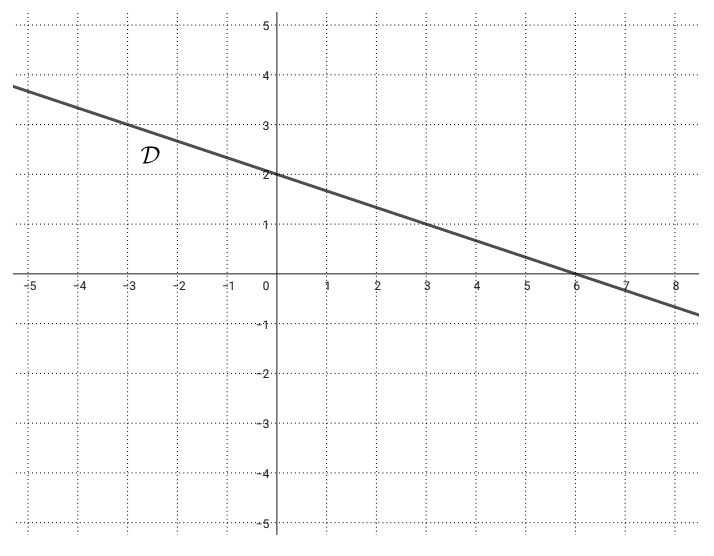
\includegraphics[width=0.8\textwidth]{fig1.png}

        \vspace{-20pt}
        \textbf{FIGURE 1}
    \end{center}

    {\color{red} \boxed{\text{$f(x) = -\dfrac{1}{3}x + 2$}}}

    \item Dans le repère de la figure 1, tracer la représentation graphique de la fonction $g$ définie sur $\mathbb{R}$ par $g(x) = \dfrac{5}{2}x - 3$.
    
    \hspace{-1.8cm}{\color{red} \boxed{\text{Je vous laisse refaire cette question par vous même avec le cours sur les fontions affines.}}}

\end{enumerate}

\section*{Exercice 5}

On considère deux fonctions $f$ et $g$ définies sur l'intervalle $[-7; 6]$ dont les représentations graphiques sont données sur la figure 2. Répondre aux questions à l'aide de lectures graphiques.

\begin{center}
    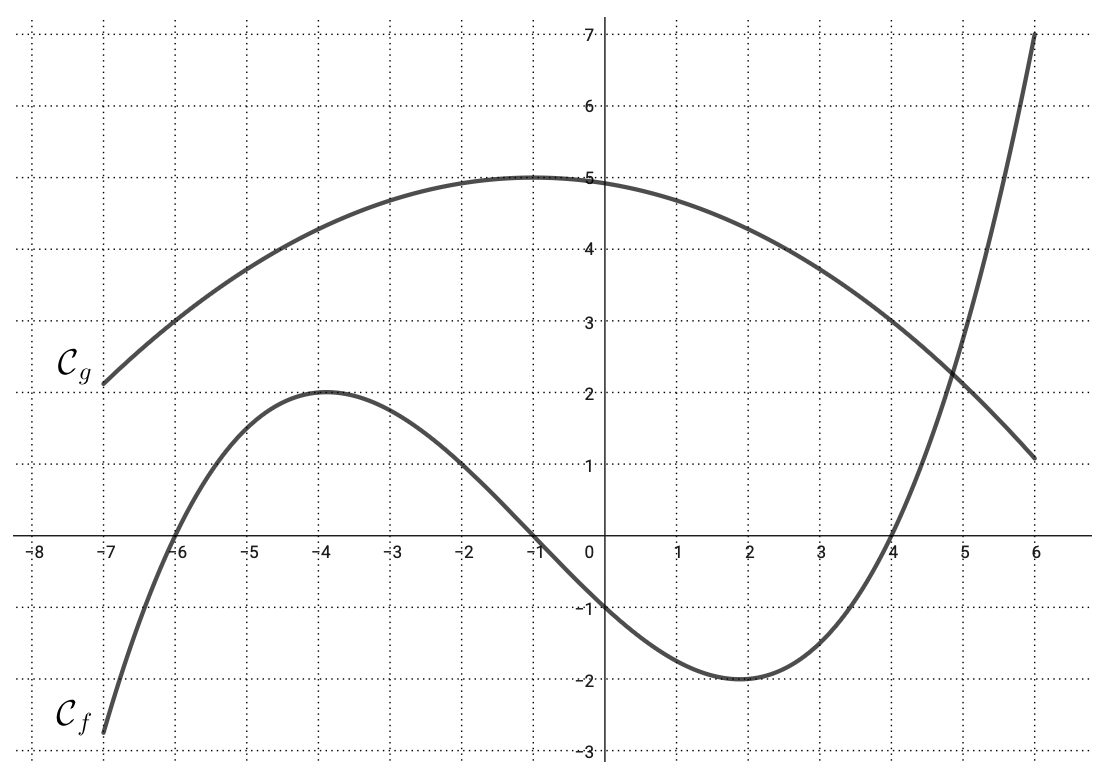
\includegraphics[width=0.8\textwidth]{fig2.png}

    \textbf{FIGURE 2}
\end{center}

\begin{enumerate}
    \item Déterminer l'image de $3$ par la fonction $g$. {\color{red} \boxed{\text{environ 3,7}}}
    \item Déterminer les antécédents éventuels de $0$ par la fonction $f$. {\color{red} \boxed{\text{-6 ; -1 et 4}}}
    \item Résoudre l'inéquation : $f(x) \leq 1$. {\color{red} \boxed{\text{$\left[-7;-5,5\right] \cup \left[-2 ; 4,4\right]$ à peu près}}}
    \item Résoudre l'inéquation : $f(x) > g(x)$. {\color{red} \boxed{\text{$\left]4,8;6\right]$}}}
    \item Dresser le tableau de signes de la fonction $f$. 
    
    \vspace{5pt}
    \hspace{-1.9cm}{\color{red}
    \begin{tikzpicture}
        \tkzTabInit{$x$ / 1 , $f(x)$ / 1}{$-7$, $-6$, $-1$, $4$, $6$}
        \tkzTabLine{, -, z, +, z, -, z, +, }
    \end{tikzpicture}
}
    \item Dresser le tableau de variations de la fonction $f$. 
    
    {\color{red} \boxed{\text{Je vous laisse refaire cette question par vous même.}}}
\end{enumerate}

\end{document}